\chapter{Grundvoraussetzungen}
Ein Auto fährt autonom auf der Autobahn, im Internet führen zwei Bots eine Unterhaltung oder der weltbeste Go-Spieler wird von einem PC geschlagen . Was haben diese scheinbar unabhängigen Ereignisse miteinander zu tun? Ihnen allen liegt eine Künstliche Intelligenz (KI) zugrunde. Um zu verstehen wie diese immer alltäglicher werdenden Phänomene überhaupt funktionieren und auf welchen wissenschaftlichen Prinzipien sie basieren, werde ich in dieser Seminararbeit, am Beispiel des Spielers des Spiels Space Invaders, eine künstliche Intelligenz entwickeln und implementieren. Diese KI soll in der Lage sein die Aktionen des Spielers auf einem niedrigen Niveau auszuführen.
\section{Künstliche Intelligenz}\label{KI}
Es ist nützlich, sich bevor man anfängt zu Programmieren, zu überlegen was KI überhaupt bedeutet.\\
Generell kann man sagen, dass es keine eindeutige Definition für künstliche Intelligenz gibt. Ein Problem dieser Mehrdeutigkeit besteht in der Tatsache, dass selbst menschliche Intelligenz schwer definierbar ist. So wird sie \glqq als Fähigkeit beschrieben, bestimmte Ziele zu erreichen \grqq \cite[S.11]{roser2021charakterisierung}. Dies bedeutet nun für den Agenten in meinem Fall, dass dieser in der Lage sein muss Space Invaders spielen zu lernen, um als intelligent zu gelten. Da diese Fähigkeit jedoch unglaublich spezifisch ist, wird oftmals  in \glqq schwache\grqq{}  und \glqq starke\grqq{} künstliche Intelligenz unterschieden. Die\glqq schwache\grqq{}  künstliche Intelligenz beschränkt sich dabei auf einen Bereich, während im Gegensatz dazu, die starke KI bereichsübergreifend agieren kann \cite[vgl.][S.11]{roser2021charakterisierung}. Somit zählt die in \ref{NN} entwickelte KI des Spielers zur schwachen KI.\\
\section{Space Invaders}
Bevor man nun aber eine künstliche Intelligenz implementiert, lohnt es sich zuerst einen Blick auf die Umgebung zu werfen in dem der Spieler agiert. Da das originale Space Invaders von 1978 ein Arcadegame ist \cite[vgl.][]{1978}, basiert meine Version auf dem Code Christian Thompson \cite[vgl.][]{Thompson2015}, die in der Programmiersprache Python geschrieben ist.
\begin{center}
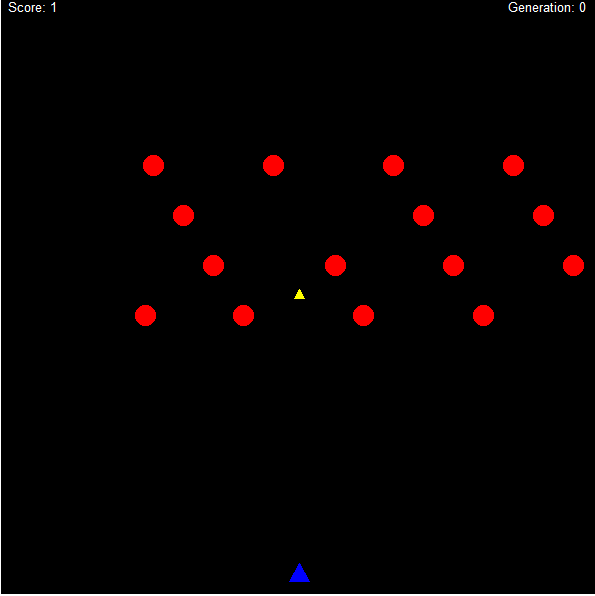
\includegraphics[scale=0.85]{Bilder/Screenshot (40)}\\
\begin{small}
\textit{Ein Screenshot von meiner Space Invaders Version}
\end{small}
\end{center}
 Wie man im obigen Bild erkennen kann, ist meine Version eher minimal gehalten, sodass nur die wichtigsten Informationen dargestellt werden. Dies ist zum Einen der Fall, um Rechenleistung zu sparen, zum Anderen macht das visuelle Erscheinungsbild für die künstliche Intelligenz (KI) später keinen Unterschied. Dies liegt an der Art der Daten, welche die KI übermittelt bekommt. Um Rechenleistung und Zeit zu sparen, ist es deshalb sinnvoll, die grafische Darstellung des Trainings zu deaktivieren\footnote{Auf das Training wird in \ref{OptF} noch genauer eingegangen}\footnote{In main.py mit grafische Darstellung änderbar}.\\ Zurück zum Aufbau, der Spieler ist das blaue Dreieck, die roten Kugeln die Gegner und das gelbe, kleine Dreieck die Kugel.\\ Der Spieler hat mehrere Handlungsoptionen: \\
 Er kann sich nach links oder rechts bewegen, nichts tun oder schießen. Falls er sich dafür entscheidet zu schießen, bewegt sich das gelbe Dreieck, die Kugel, senkrecht nach oben. Es ist aber immer nur eine Kugel im Spiel, dass heißt wenn der Spieler schießt und es ist schon eine Kugel im Spiel, passiert nichts. Die Kugel wird zurückgesetzt, wenn sie entweder einen Gegner trifft oder das Spielfeld verlässt.\\ Von den Gegnern hingegen existieren standardmäßig 16 Instanzen\footnote{Mit self.Monsterzahl veränderbar}. Sie bewegen sich von einem Spielfeldrand zum Anderen. Wenn ein Gegner den Rand erreicht, werden alle Gegner eine Reihe nach unten gesetzt und ihre Bewegungsrichtung ändert sich. Sie gewinnen, wenn ein Gegner unterhalb des Spielers ist. Im Gegensatz dazu, gewinnt der Spieler, wenn kein Gegner mehr existiert. Damit ein Gegner geschlagen wird, muss ihn die Kugel treffen\footnote{Wird mit isCollision() überprüft}.\\
Im weiteren Verlauf dieser Seminararbeit werde ich nun versuchen den Spieler des Spiels Space Invaders durch eine KI zu steuern. Dafür werde ich  verschiedene Möglichkeiten, wie Bestärkendes Lernen (Reinforcement Learning/ RL) oder Entscheidungsbäume, betrachten, um zu diese Aufgabenstellung zu lösen. Bei Beispielen werde ich mit Fußnoten darauf zu verweisen, wo das aktuell Diskutierte im Code zu finden ist.

\chapter{Bestärkendes Lernen }
Das bestärkende Lernen, auch Reinforcement Learning genannt, ist neben dem überwachten Lernen und dem unüberwachten Lernen eine der Möglichkeiten des maschinellen Lernens . Es versucht aus den gegebenen Daten, ohne anderes  vorhergehendes Wissen, Informationen zu gewinnen\cite[vgl.][S.7]{li2017deep}.
\label{NN}
\section{Funktionsweise}
\begin{center}
 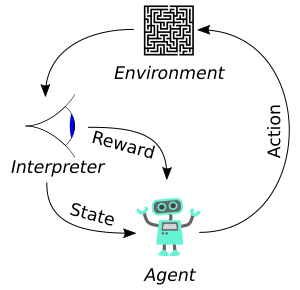
\includegraphics[scale = 1]{Bilder/Reinforcement_learning_diagram}\\
 \small{\textit{The typical framing of a Reinforcement Learning scenario}}\cite{RLdia}
\end{center}
Auf der Darstellung kann man die typische Funktionsweise des Bestärkenden Lernens erkennen.  Der Agent, führt eine Aktion aus, welche seine Umwelt (enviroment) beeinflusst. Daraufhin bekommt dieser wiederum die Information über den neuen Zustand (state) der Umwelt  und eine Belohnung (reward), die auch negativ sein kann. Diese Schleife kann nun unendlich oft wiederholt werden. Für den Spieler im Projekt bedeutet das, dass er eine Aktion (Schuss, Linksbewegen oder Rechtsbewegen) ausführen kann und daraufhin die neuen Koordinaten der Gegner sowie den neuen Punktestand, für dessen Steigen er gleichzeitig eine Belohnung erhält, mitgeteilt bekommt.   
\section{Neuronales Netz}

Ein künstliches neuronales Netzwerk, ist ein Modell des zentralen Nervensystems, welches lernt auf Informationen zu reagieren. Wie das Gehirn aus verschiedenen Nervenzellen aufgebaut ist, besteht das Neuronale Netz aus künstlichen Neuronen, welche in verschiedenen Schichten verknüpft sind, wie im nächsten Unterkapitel ausgeführt wird. Ein nicht zu vernachlässigender Unterschied von künstlichen neuronalen Netzen im Vergleich zu dem menschlichen Gehirn besteht in der Anzahl der Verknüpfungen. Denn während unser Gehirn ca. $10^{14}$ Verknüpfungen beinhaltet, haben selbst die größten künstlichen neuronalen Netzwerke nur einen Bruchteil der Verbindungen (ca. 100.000) \cite[vgl.][S.1055]{traeger2003kunstliche}. Eine Konsequenz dieser limitierten Größe besteht zum Beispiel darin, dass es noch keine  KI gibt, die alle Aufgaben lösen kann.  
\subsection{Topologie}
Topologie bezeichnet in Zusammenhang mit Neuronalen Netzen die Struktur des Netzes, also die Anordnung der Neuronen und deren Verbindungen untereinander.
% todo : Upadte dimensions of Neural Network
\begin{center}


\begin{neuralnetwork}[height=6]
        \newcommand{\x}[2]{$x_#2$}
        \newcommand{\y}[2]{$\hat{y}_#2$}
        \newcommand{\hfirst}[2]{\small $h^{(1)}_#2$}
        \newcommand{\hsecond}[2]{\small $h^{(2)}_#2$}
        \newcommand{\hthird}[2]{\small $h^{(3)}_#2$}
        \inputlayer[count=3, bias=true, title=Eingabe\\Schicht, text=\x]
        \hiddenlayer[count=6, bias=false, title=Verdeckte\\Schicht 1, text=\hfirst] \linklayers
        \hiddenlayer[count=6, bias=false, title=Verdeckte\\Schicht 2, text=\hsecond] \linklayers
         \hiddenlayer[count=6, bias=false, title=Verdeckte\\Schicht 3, text=\hthird] \linklayers
        \outputlayer[count=4, title=Ausgabeschicht, text=\y] \linklayers
    \end{neuralnetwork}\\
    \small{\textit{Nicht die Größe des im Projekt verwendeten Neuronalen Netzes}}
    \end{center}
    Auf der Abbildung oben erkennt man das Modell eines Neuronales Netzes mit einer Eingabeschicht mit 4 Eingabewerten, 3 verdeckten Schichten mit jeweils 6 Neuronen und einer Ausgabeschicht mit 4 Neuronen. Ebenfalls erkennt man, dass es sich bei der Art des Neuronalen Netzes um ein Feedforward Netz handelt, da die Daten von den Neuronen an die Neuronen der darauffolgenden Schicht weitergegeben werden.\footnote[5]{In der Programmierung wird die Größe des Neuronalen Netzes mit der Methode HiddenLayers(AnzahlHiddenLayers) festgelegt}
\subsection{Künstliche Neuronen}
Wie oben schon genannt bestehen Neuronale Netze aus künstlichen Neuronen, welche natürlichen nachempfunden sind.\begin{center}


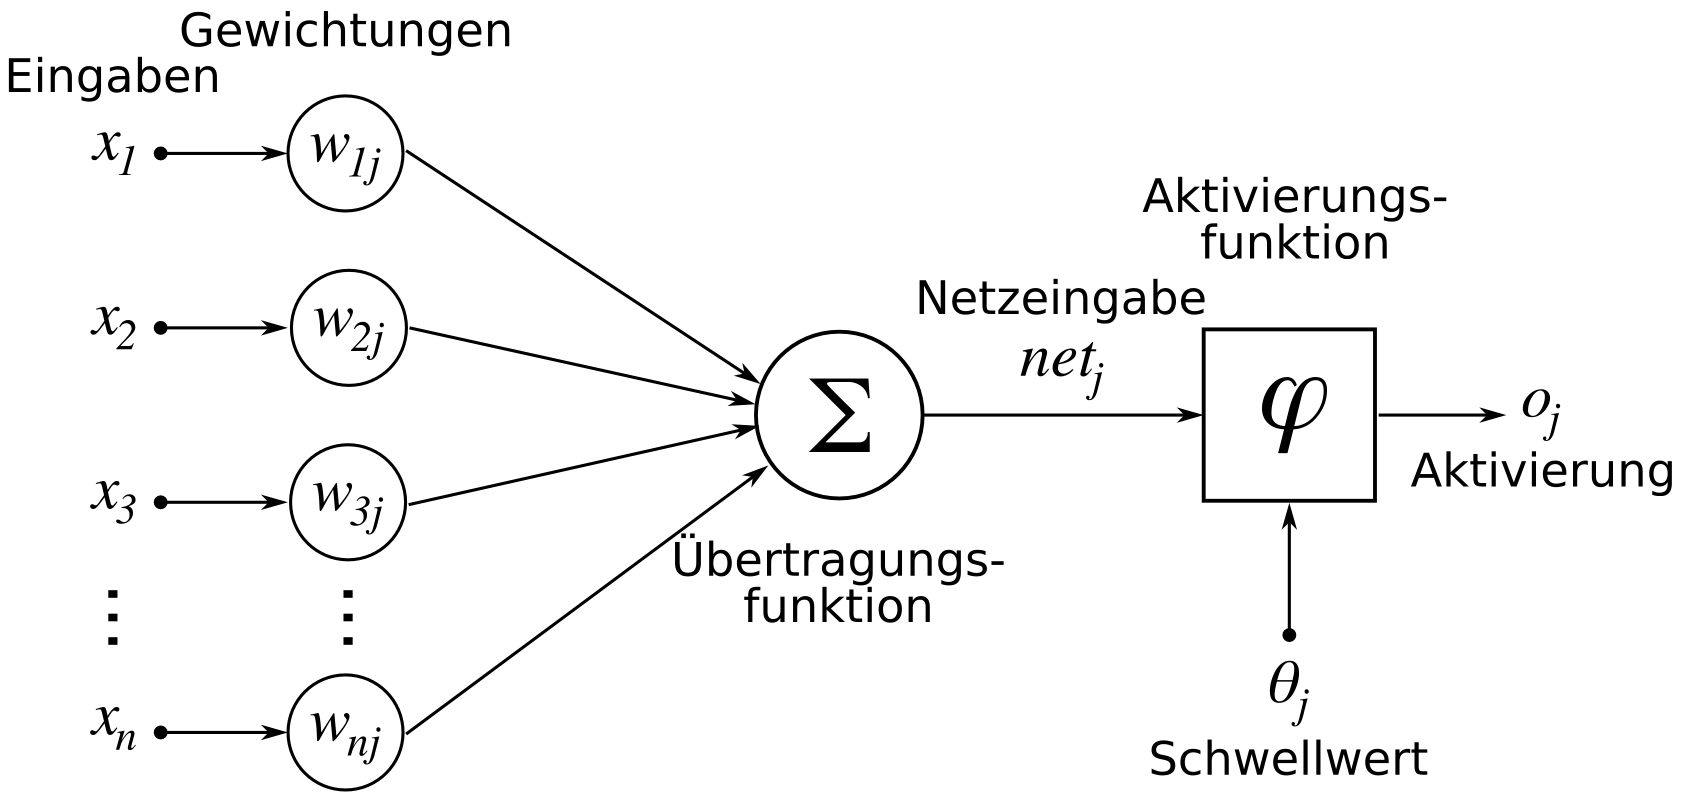
\includegraphics[width=0.8\textwidth]{Bilder/ArtificialNeuronModel_deutsch.png}\cite{das}\end{center}
Wie man auf der Abbildung erkennen kann wird in einem künstlichen Neuron die Summe der Produkte aus Gewichten und Eingaben durch die Aktivierungsfunktion zur nächsten Eingabe.
\subsubsection*{Aktivierungsfunktion}

	Aktivierungsfunktionen werden dazu benutzt um die Information einer Schicht des neuronalen Netzwerks zu verarbeiten um sie an die nächste Schicht weiterzugeben.\\

	Das Benutzen einer Aktivierungsfunktion ist von Vorteil, da so dem Neuronalen Netzwerk ermöglicht wird, komplexere Probleme zu lösen. Ein Neuronales Netz ohne Aktivierungsfunktion zu trainieren ist trotzdem möglich, es könnte aber nur lineare Probleme lösen.
	%todo : Einfügen warum Modell nicht linear ist
	
	Deshalb werden im Maschinellen Lernen, wenn es mehrere verdeckte Schichten gibt oftmals Aktivierungsfunktionen benutzt.\\
	
\subsubsection*{Sigmoidfunktion} \label{Sig}
	Die Sigmoidfunktion ist die am häufigsten benutzte Aktivierungsfunktion, da sie eine nicht lineare Funktion ist. Sie kann folgendermaßen beschrieben werden:
	\begin{center}
	\large{f(x)= $\frac{1}{1+e^{-x}}$}
	
	\end{center}

Im Projekt wurde diese Sigmoidfunktion ebenfalls verwendet, da sie nicht linear ist, die Werte in einen Bereich zwischen 0 und 1 transformiert und ableitbar ist \cite[vgl.][S.312 Abschnitt c]{sharma2017activation}.\\
\begin{center}


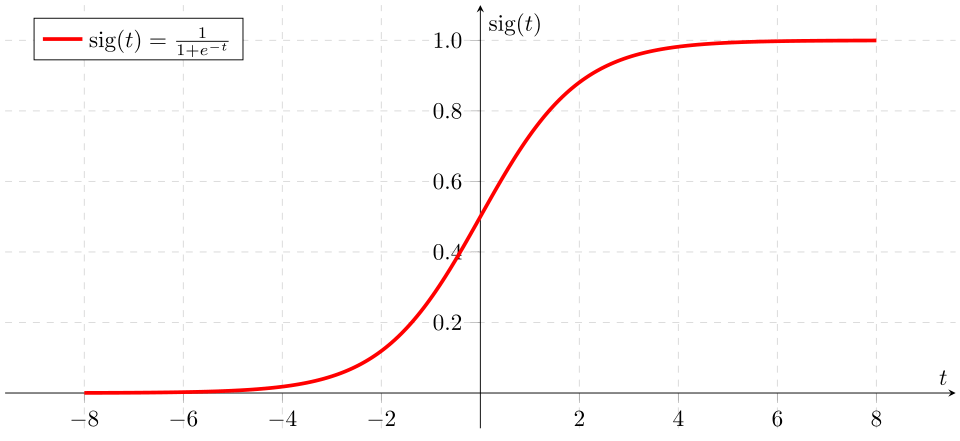
\includegraphics[width=0.8\textwidth]{Bilder/Sigmoid-function-2.png}\\
%todo
\small{\textit{Plot der Sigmoidfunktion im Intervall }[-8;8]\tab \cite{MartinThoma2014}}
\end{center}
Für zu große x-Werte kann es in Python zu einem \glqq Overflow Error" kommen. In diesem Fall wird f(x) zu Null wenn x kleiner 0 ist und zu Eins wenn x größer 0 ist. 
\section{Optimierungsfunktion}
Die Optimierungsfunktion ist im Projekt der Algorithmus, der die Gewichte des Neuronalen Netzes anpasst\footnote[6]{Im Projekt die Methode: evaluieren(score)} nach der Form:\\
\begin{center}


\textit{Reward Increment = Nichtnegativer Faktor * Offset Reinforcement * Characteristic Eligibility} \cite[vgl.][S.234]{williams1992simple}\\ \textbf{oder}
\\
$\Delta w_{ij} = \alpha _{ij}(r-b_{ij})e_{ij}$\\
\end{center}
Wobei $\Delta w_{ij}$ die Gewichtsänderung darstellt, der nicht negative Faktor $\alpha _{ij}$ auch eine Konstante sein kann, die auch als Lernfaktor bekannt ist\footnote[7]{Im Projekt: self.Lernfaktor = 3}, der Minuend \textit{r} die aktuelle Punktzahl, der Subtrahend \textit{b} die maximale Punktzahl aller Generationen und $e_{ij}$ ein Produkt
$e_{ij} =ln(f_{ij})\cdot{}\dfrac{1}{w_{ij}}$ mit $f_{ij}$, dem durch die Aktivierungsfunktion berechneten Ausgabe eines Neurons und $w_{ij}$ dem derzeitigen Gewicht des Neurons.\\
Diese Funktion hat jeden Durchgang eine Chance\footnote[8]{ In der Methode maingameloop() mit der lokalen Variable \textit{ch} änderbar} aufgerufen zu werden, um das Neuronale Netz zu aktualisieren.\label{OptF}
\subsubsection*{Probleme der Optimierungsfunktion}
Wenn \textit{b} gleich \textit{r} wird die ganze Gleichung 0, somit kann kein weiteres Lernen mehr stattfinden.

\section{Probleme des Bestärkenden Lernens}
Beobachtet man den maximalen Score des Spielers in der derzeitigen Konfiguration über mehrere Generationen und Anläufe hinweg, so stellt man fest, dass dieser selten, wenn nicht sogar nie, über 5 Punkte hinausgeht. Daher muss ich nach den Problemen suchen, die verhindern, dass der Agent mehr lernt.
\subsection{Underfitting}
Underfitting (deutsch Unteranpassung) ist ein Problem, das im bestärkenden Lernen auftreten kann, wenn das Modell weniger komplex ist, als die Daten mit denen es zu arbeiten versucht\cite[vgl.][S.6-7]{koehrsen2018overfitting}. Dies ist zu Beispiel der Fall, wenn man versucht ein lineares  Modell auf ein nicht lineares Problem anzuwenden. Dies ist bei dem hier verwendeten Neuronalen Netzwerk nicht der Fall, da die in \ref{Sig} beschriebene Aktivierungsfunktion nicht linear ist und somit das Modell komplex genug sein sollte, um Space Invaders zu schlagen.

\subsection{Overfitting}
Was eher der Fall sein könnte, ist eine Art des sogenannten Overfittings, das im Deutschen als Überanpassung bekannt ist. Hierbei passt der Agent seine Strategie zu genau an das Problem an und probiert keine neuen Strategien mehr aus. Dieser Fall tritt hier ein, wenn der Spieler lernt nur zu schießen, weil er damit eine Punktzahl von 5 erreicht und diese höher ist als die vorherige Punktzahl. Eine Möglichkeit, dieser Überanpassung vorzubeugen, besteht darin, das Problem leicht zu variieren. Zum Beispiel kann man die Gegner jede Runde zufällig platzieren.\footnote[9]{ Dies passiert wenn man in der reset-Funktion die lokale Variable  random auf False setzt}. Dies kann aber auch zur Folge haben, dass der Agent das Problem zufällig löst. Auch könnte dieses Problem gelöst werden, indem man die Belohnung an die vergangene Zeit koppelt, ähnlich wie ich noch in \ref{D1} erklären werde.

\chapter{Alternativen zum Bestärkenden Lernen}\label{AL}
\sectionmark{Alternativen zu RL}
Die in \ref{KI} aufgestellte Definition von Künstlicher Intelligenz wirft aber die Frage auf, wo künstliche Intelligenz überhaupt beginnt. Um diese Frage zu beantworten, werden in \ref{AL} nun zwei Alternativen zum Bestärken Lernen vorgestellt.\\
Eine weitere Idee, eine Künstliche Intelligenz zu trainieren, welche sich nicht auf ein neuronales Netz stützt, besteht darin, Entscheidungsbäume zu verwenden. Da das System, in welchem sich der Spieler bewegt, nicht überaus kompliziert ist, ist diese Möglichkeit durchaus machbar.
\section{Entscheidungsbäume}
%todo Definition und kleines Intro
Entscheidungsbäume zählen zu den wissensbasierten Systemen, die Wissen, das aus Beobachtungen oder Regeln besteht, speichern \cite[vgl.][S.81-82]{quinlan1986induction}. Sie sind auch oft einfacher zu verstehen, als andere Systeme, wie zum Beispiel Neuronale Netzwerke. Entscheidungsbäume sind aber manchmal so komplex, dass die wahre Herausforderung darin besteht, die Pfade zu finden, welche zum gewünschten Ergebnis führen.
\label{EB}
\subsection{Implementierung im Projekt}
\begin{center}


	\begin{sequencediagram}

		\newthread[white]{p}{Spieler:}
		\newinst[2]{b}{Baum:}
		\newinst[2]{a}{aktuellerKnoten:}
		\newinst[2]{n}{nächsterKnoten:}
			\begin{call}{p}{moveGeben(4)}{b}{r}
				\begin{call}{b}{moveGeben(4)}{a}{r}
					\begin{call}{a}{moveGeben(4)}{n}{r}
					\end{call}
				\end{call}
			\end{call}
	\label{D1} 
	\end{sequencediagram}
	\textit{\small{Sequenzdiagramm einer möglichen Aktion des Spielers}}\\
	
\end{center}
In diesem Diagramm kann man erkennen, wie der Spieler den Baum nach einer Aktion fragt. Bei der Methode moveGeben(4) drückt die 4 einen Übergabewert aus, der einen simulierten Score übergibt. Den tatsächlichen Score als Übergabewert zu benutzen ist auch möglich, aber weniger effektiv, da je früher ein Gegner zerstört wird, der nächste Gegner zerstört werden kann. Die Funktion F, die den Übergabewert errechnet, besitzt eine ähnliche Aufgabe zur Aktivierungsfunktion im Neuronalen Netz.\begin{center}
	$F(score,t_{1},t_{2})=score \cdot \dfrac{t_{2}-t_{1}}{10}$
\end{center} Der simulierte Score F wird mit der obigen Gleichung berechnet, wobei $t_{1}$ die Zeit in Sekunden zu Beginn des Durchlaufs, $t_{2}$ die Zeit in Sekunden zum Zeitpunkt der Abfrage und \textit{score} die tatsächliche Punktzahl ist.\\ %todo eleganter formulieren

Man kann diese Funktion noch verbessern, indem man den außerdem die Position des Gegners miteinbezieht, da, falls der äußerste Gegner zerstört wird, die Schritte bis zum Näherkommen der Gegner zunehmen. Somit ist es wichtiger, äußere Gegner zu zerstören, als Innere.\\
Der aktuelle Knoten vergleicht die Punktzahl seiner Kinder untereinander und gibt mit einer 19:1 Wahrscheinlichkeit den Move des Knotens mit der höchsten Punktzahl zurück.
\subsubsection*{Objektdiagramm}
\begin{center}



	\begin{tikzpicture}[node distance = 2cm]
		\node (Spielkonsole)[objekt, rectangle split, rectangle split parts=2]
		{			
			\textbf{Spielkonsole}
			\nodepart{second}self.Art ="Baum"\\ self.Baum = Baum
		};
		\node (Baum)[objektb, rectangle split, rectangle split parts=2, right =of Spielkonsole]
		{			
			\textbf{Baum}
			\nodepart{second}self.wurzel = K1
			\\self.aktuellerKoten = K2
		};
		\draw[myarrow](Spielkonsole) -- (Baum);
		\node (K1)[objektb, rectangle split, rectangle split parts=2, below = of Baum]
		{			
			\textbf{K1}
			\nodepart{second}self.Kinder =[K2,K3,K4,K5]\\ self.score = 0 \\ self.move = None \\ 
		};
		\draw[myarrow](Baum) -- (K1);
		   \node (AuxNode01) [text width=0cm, below=of K1] {};
		 \node (K3)[objekts, rectangle split, rectangle split parts=2, left =0.5cm of AuxNode01]
		{			
			\textbf{K3}
			\nodepart{second}self.Kinder = [ ]\\ self.score = 0 \\ self.move =  \dq l \dq{} \\ 
		};
		\node (K2)[objekts, rectangle split, rectangle split parts=2, left =1cm of K3]
		{			
			\textbf{K2}
			\nodepart{second}self.Kinder = [ ]\\ self.score = 0 \\ self.move = \dq r \dq{} \\ 
			
		};
		\node (K4)[objekts, rectangle split, rectangle split parts=2, right =0.5cm of AuxNode01]
		{			
			\textbf{K4}
			\nodepart{second}self.Kinder = [ ]\\ self.score = 0 \\ self.move = \dq s \dq{} \\ 
		};
		\node (K5)[objektm, rectangle split, rectangle split parts=2, right =1cm of K4]
		{			
			\textbf{K5}
			\nodepart{second}self.Kinder = [ ]\\ self.score = 0 \\ self.move = None \\ 
			
		};
	\draw[myarrow](K1) -- (K2);\draw[myarrow](K1) -- (K3);\draw[myarrow](K1) -- (K4);\draw[myarrow](K1) -- (K5);
	\end{tikzpicture}
	\textit{\small{Objektdiagramm, dass einen Ausschnitt eines Baums zeigt}}
\end{center}
Wie im Sequenzdiagramm in \ref{D1} schon erläutert, werden die Aktionen des Spielers durch eine rekursive Methode ermittelt. Diese vergleicht die Punktzahlen der Kinder des aktuellen Knotens und die Aktion des Kindes mit der höchsten Punktzahl, mit einer Wahrscheinlichkeit von 95\% zurückgibt.\\ Was passiert aber, wenn keine Kinder vorhanden sind oder der 20ste Fall eintritt?\\ In beiden Fällen wird zufällig eine Aktion ausgewählt und zurückgegeben. Im ersten Fall müssen zusätzlich noch Kinder erzeugt werden. 
\subsection{Probleme und Einschränkungen}
Eine Beobachtung, welche ich im Laufe der Testläufe des Programms gemacht habe, besteht darin, dass die zufällige Art des Entscheidens, die ich verwendet habe, nur dann funktioniert, wenn die Gegneranzahl relativ klein ist (ca. 12).%todo

Ein weiteres Problem, das mir bei meiner Implementierung im Weg stand, besteht im Speicherplatzverbrauchs des Baums. Denn während ein Neuronales Netz eine fixe Größe hat, nimmt die des Baums stetig zu. So hat zum Beispiel ein Baum nach vier Aktionen des Spielers vier Knoten und nach 16 Aktionen 16 Knoten. Im Gegensatz dazu bleibt die Größe eines künstlichen neuronalen Netzes konstant. Hinzu kommt ebenfalls, dass nicht alle  Pfade im Baum sinnvoll sind, weil sie zum Beispiel das Gleiche aussagen.\\ Folgendes Beispiel:\\
\begin{center}


	\begin{tabular}[h]{r|c|c|c|c}
		 & 1 & 2 & 3 & 4\\
		\hline
		Aktion des Spielers & - & r & - & r\\
		\hline
		Alternativ & r & r & - & -\\

	\end{tabular}\\
	\textit{\small{ r $\stackrel{\wedge}{=}$ Schritt nach rechts; - $\stackrel{\wedge}{=}$ keine Bewegung}}
	%todo Verbessern
	\end{center}
	

Auf dieser Tabelle sieht man, dass es mehrere Aktionsabfolgen des Spielers gibt, welche zum exakt gleichen Ergebnis führen. In diesem Fall bewegt sich der Spieler zwei Schritte nach rechts. Die Abfolge der Aktionen ist in diesem Fall egal, da nur die Position des Spielers zum Zeitpunkt eines Schusses einen Unterschied auf das Ergebnis macht.
\subsection{Lösungsmöglichkeiten}
Einige Maßnahmen die zur Verbesserung des Baumes getroffen werden können, werden im Folgenden aufgezählt und kurz erläutert:\\
	\begin{itemize}
	\item Man kann Pfade, welche nicht zum Ergebnis führen, trimmen (prunen) \cite[vgl.][S.72]{quinlan}, indem man beispielsweise den Pfad durch ein einzelnes Blatt ersetzt. Dies führt dazu, dass Speicherplatz frei wird, der dann wiederum für neue Pfade genutzt werden kann.% Für Gewöhnlich basieren diese Pruningtechniken auf Kosten-Komplexität Modellen, pessimistischen Genauigkeitseinschätzungen oder auf der Minimierung der Nachrichtenlänge, die den Baum samt Daten beschreibt. can be included if optimized
	\item Auch können mehrere Bäume zu Einem zusammengefügt werden, wodurch sich die Komplexität des Baumes vergrößert, indem nun in diesem Baum mehr Pfade enthalten sind\cite[vgl.][S.72]{quinlan}. Dies trägt in meinem spezifischen Fall aber nicht zur Lösung des Problems des begrenzten Speicherplatzes bei. Im Gegenteil, es verstärkt dieses Problem nur weiter, weil der neue Baum komplexer ist und somit mehr Speicherplatz verbraucht.
	\item Indem man in einem bestehenden Baum neue Pfade einfügt, anstatt immer wieder den kompletten Baum nach einem Durchlauf des Programms neu zu Generieren, verringert die Zeit, welche zum Generieren neuer Pfade benötigt wird \cite[vgl.][S.72]{quinlan}
	\end{itemize} %todo vlt andere Quellen suchen
		  
\section{Ein einfacher Algorithmus}
Alternativ könnte man auch einfach selbst einen Algorithmus schreiben mit dem die Aktionen des Spielers bestimmt werden können, wie folgendes Minimalbeispiel in Pseudocode:\\
\begin{center}


 def moveGeben(x):\\
	\tab if x $<$ -180:\\
		\tab \tab  shoot()\\
	\tab else:\\
		\tab \tab  moveleft() \\
		\label{algor}
		\end{center}
Natürlich wird dieses Minimalbeispiel nicht funktionieren, wenn es eine mittlere bis große Anzahl an Gegnern gibt. Da aber die Position der Gegner, die Gegnergeschwindigkeit, die Kugelgeschwindigkeit, sowie die Spielerposition bekannt sind, könnte man ein Gleichungssystem aufstellen. Dieses berechnet dann, wann der Spieler wo schießen muss, um einen Gegner zu treffen. Falls die Gegneranzahl dann so groß ist,das diese verbesserte Version aufhört zu funktionieren, kann man weitere Parameter, wie die Reihenfolge mit der die Gegner abgeschossen werden sollen, einführen.\\ Somit kann dieser Ansatz unter Miteinbeziehung aller möglichen Parameter auch ohne Lernfähigkeit effektiver sein, als jede mögliche Künstliche Intelligenz.
\section{Fazit}
Während der in \ref{EB} vorgestellte Entscheidungsbaum und der dazugehörige Algorithmus  meine Kriterien für künstliche Intelligenz erfüllen, nämlich Lern- und Problemlösungsfähkeit ( wenn auch nur für geringe Gegnerzahlen), ist der Algorithmus, selbst bei der losesten Definition von Künstlicher Intelligenz nicht intelligent, da die Lernfähigkeit fehlt. Ich habe ihn trotzdem aufgenommen um aufzuzeigen, dass es keiner Neuronalen Netze oder Entscheidungsbäume bedarf um die einfache Aufgabe, Space Invaders zu schlagen, zu meistern. Ein weiterer Aspekt, in dem sich Algorithmus und Künstliche Intelligenz unterscheiden, wird deutlich, wenn man den letzten Satz aus \ref{algor} betrachtet: \glqq Somit kann dieser Ansatz unter Miteinbeziehung aller möglichen Parameter auch ohne Lernfähigkeit effektiver sein, als jede mögliche Künstliche Intelligenz\grqq . Besonders auf den Teil der \glqq \textit{ Miteinbeziehung aller möglichen Parameter}\grqq{} möchte ich aufmerksam machen, da es in der wirklichen Welt zu viele Parameter gibt, als das diese alle in einem Modell berücksichtigt werden können.
\chapter{Schlussgedanken}
Wenn man die Zeit, welche ich dafür verwendet habe ein funktionierendes Neuronales Netzwerk zu entwickeln und programmieren, mit der Zeit gegenüberstellt, die für ich den Algorithmus in \ref{algor} gebraucht habe, so stellt man fest, das die eine Aufgabe über 20 Stunden und die andere nur um die 5 Minuten gedauert hat. Dabei ist das Ergebnis der einfacheren Aufgabe besser , als das der Komplizierteren. Folglich kann man daraus schließen, dass man für eine einfache Aufgabe, wie das Computerspiel Space Invaders zu schlagen, keine komplizierten Methoden anwenden sollte. Stattdessen sollte man die Methoden verwenden, die am schnellsten zum Ziel führen. Man muss auch bedenken, dass diese einfacheren Methoden einfacher zu verbessern, warten und auch verständlicher sind. Im Nachhinein hätte das Ziel für meine Seminararbeit nicht lauten sollen: \glqq Versuch etwas Neues, dass noch niemand getan hat\grqq{}, sondern  \glqq Benutze das, von dem du weißt, es funktioniert\grqq{}.\\
Zudem bin ich einige Tage vor der Abgabe auf OpenAI Gym gestoßen \cite[vgl.][]{1606.01540}. Ein Projekt auf den man seine KI unkompliziert implementieren und verschiedene Lernalgorithmen miteinander vergleichen kann. Leider funktioniert die Bibliothek, welche dafür verwendet wird, nur auf LINUX und MacOs, aber nicht Windows, das ich benutze, ansonsten hätte ich eine einfache Möglichkeit mein Projekt mit  Anderen zu vergleichen.\\ \\ Falls man etwas von dieser Seminararbeit mitnehmen sollte ist es Folgendes: Ein Auto kann autonom fahren, zwei Bots können eine Unterhaltung führen oder der weltbeste Go-Spieler kann von einem PC geschlagen werden. Dabei darf man aber nicht vergessen, dass alle diese Fortschritte erst durch menschliche Intelligenz ermöglicht wurden. Somit sollte man diese Errungenschaften nicht der KI zusprechen, sondern deren Erschaffern.